\section{General Idea}

\begin{figure}
\centering
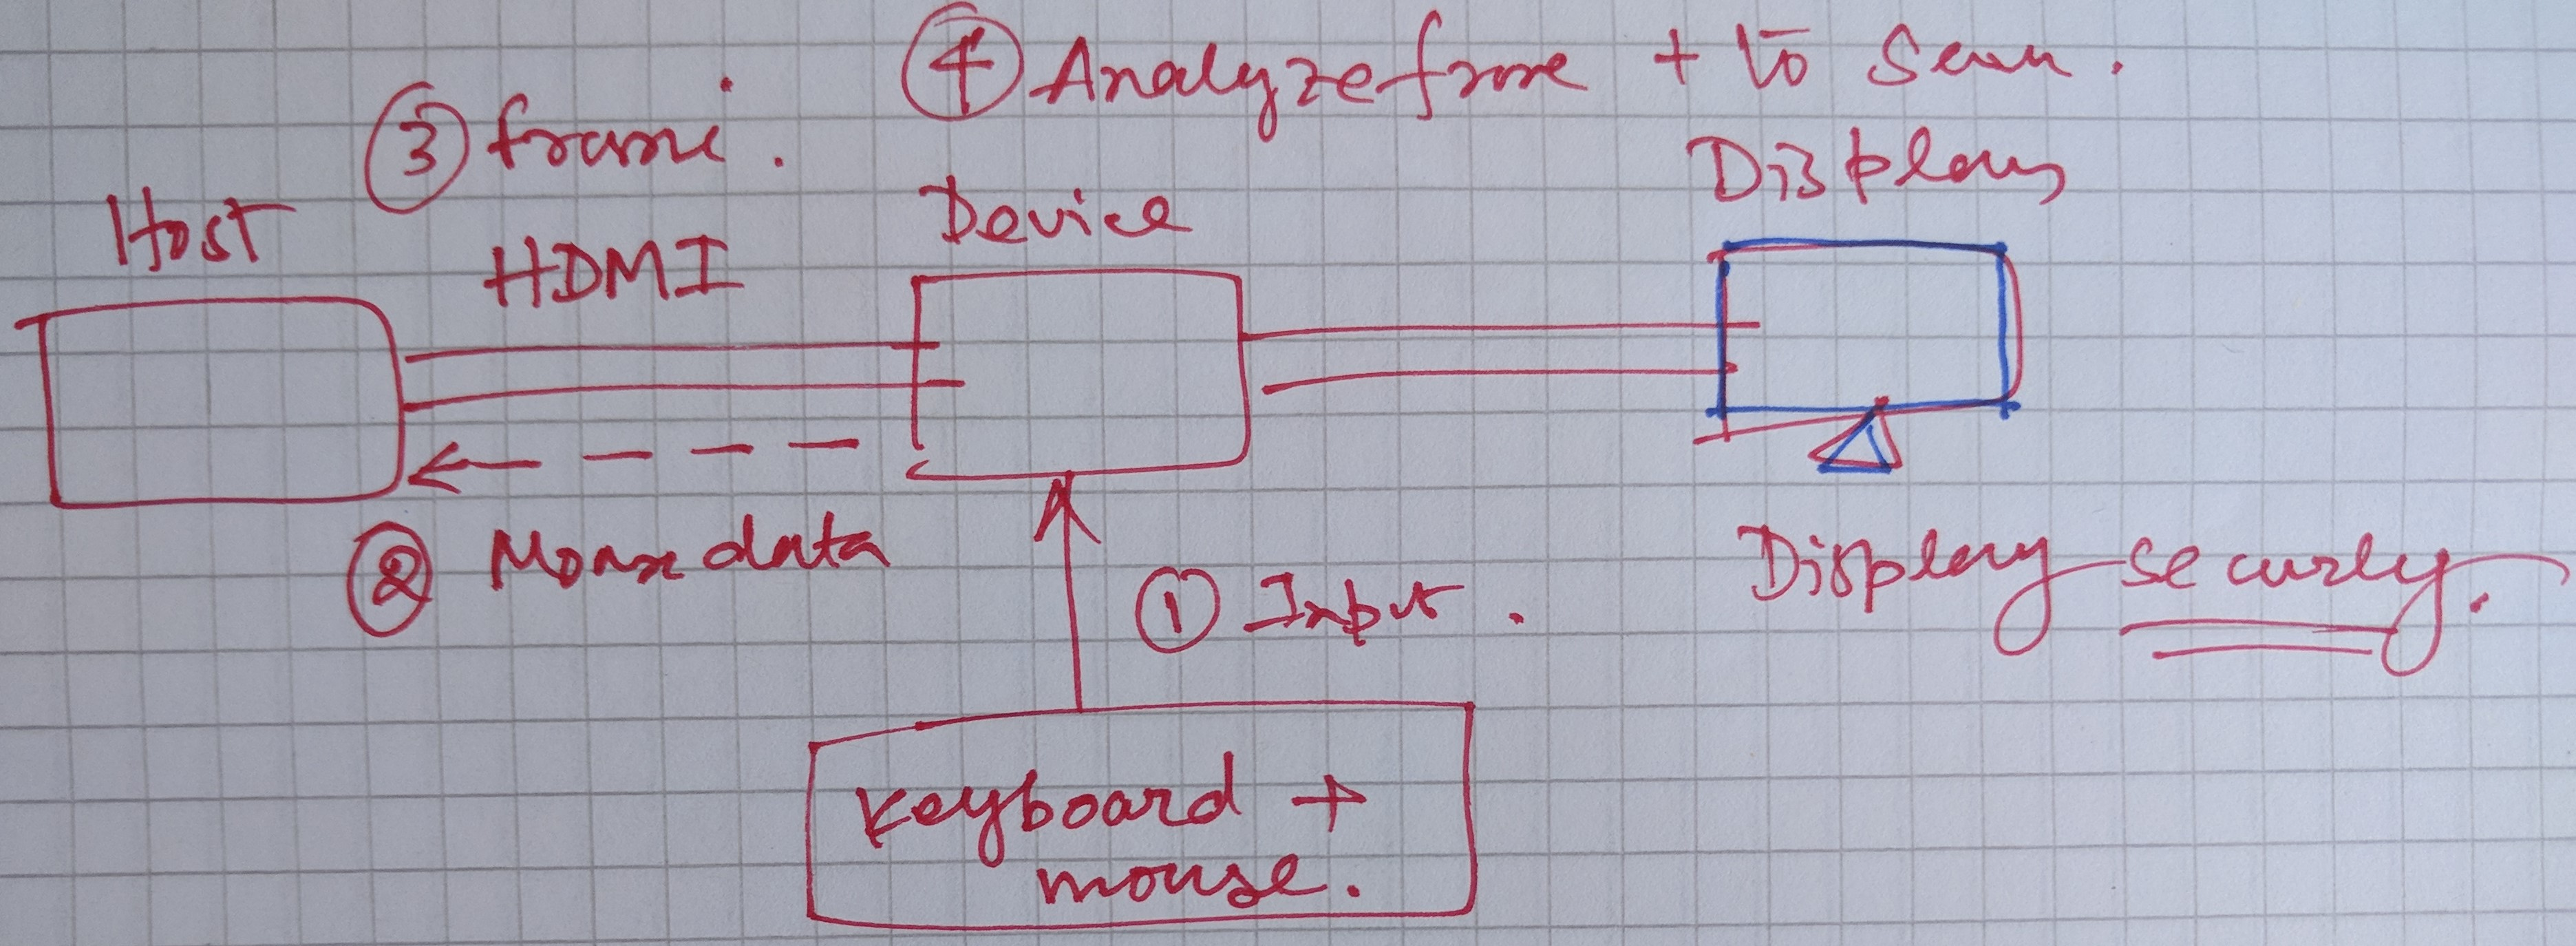
\includegraphics[width=\linewidth]{overall.jpg}
\caption{Overall Idea}
\label{fig:overallIdea}
\centering
\end{figure}


Figure~\ref{fig:overallIdea} provides the overall system design of \name. The components of the systems are the following:

\begin{enumerate}
  \item \textbf{\device.} The \device is connected to the input devices and sits between the host and the display. The \device is connected to the input devices over \usb interface and conncected to the host and the display over HDMI.
  \item \textbf{Input device.}
  \item \textbf{Display.}
  \item \textbf{Host system.}
\end{enumerate}

The steps are the following:

\begin{enumerate}
  \item The user provides input from her input device which is captured by the \device.
\end{enumerate}


\begin{figure}
\centering
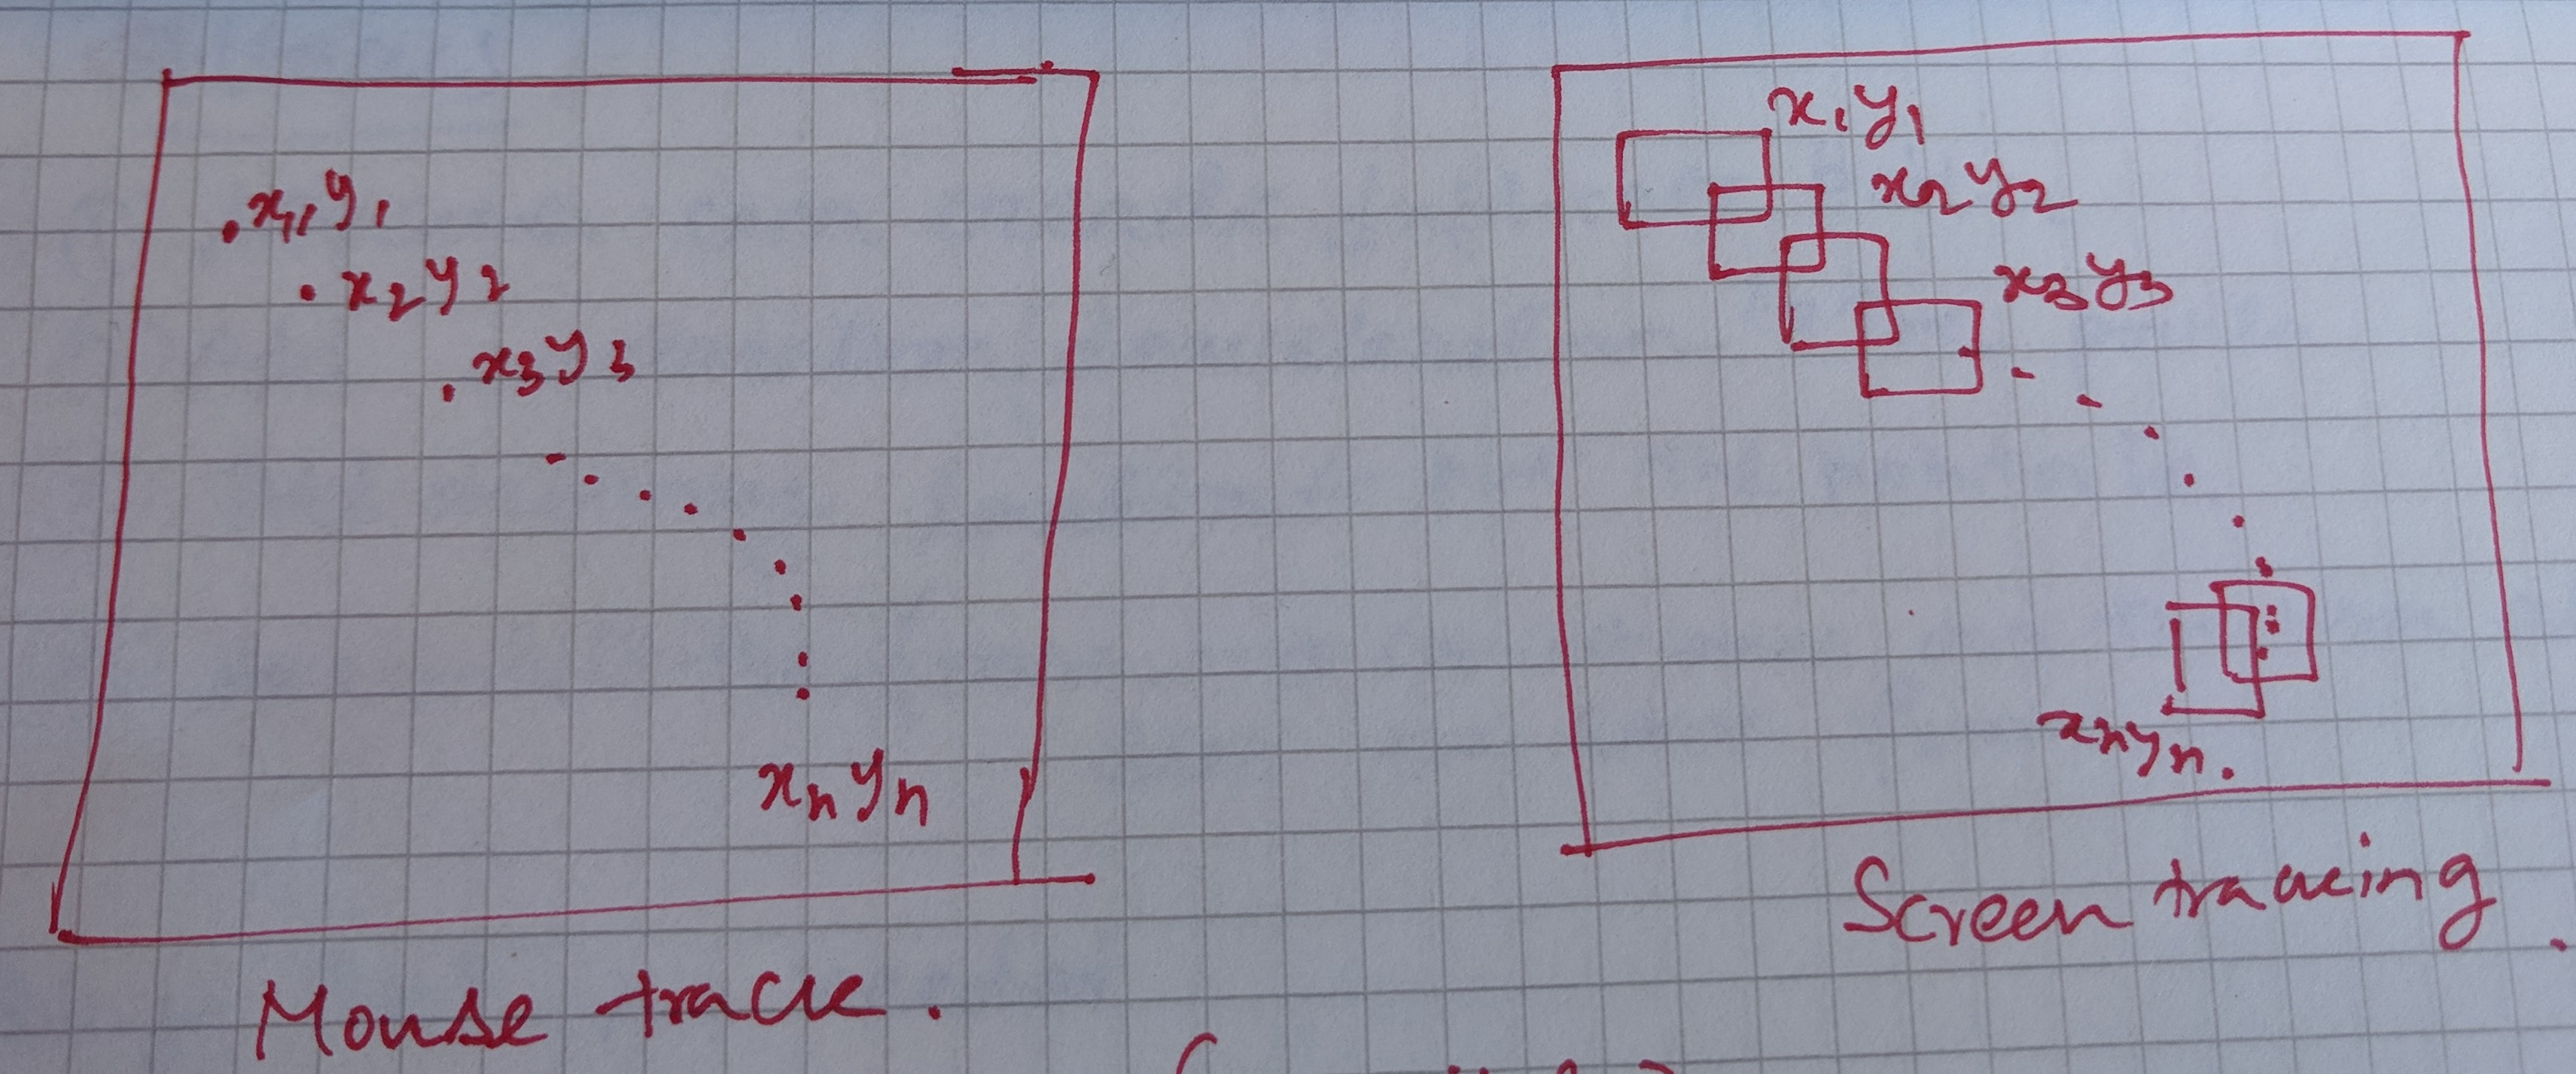
\includegraphics[width=\linewidth]{mouse_track.jpg}
\caption{}
\label{fig:overallIdea}
\centering
\end{figure}

